

\chapter{Supplements to Chapter 5}\label{appendix:a5}





\begin{figure}[htb!]
	\centering
	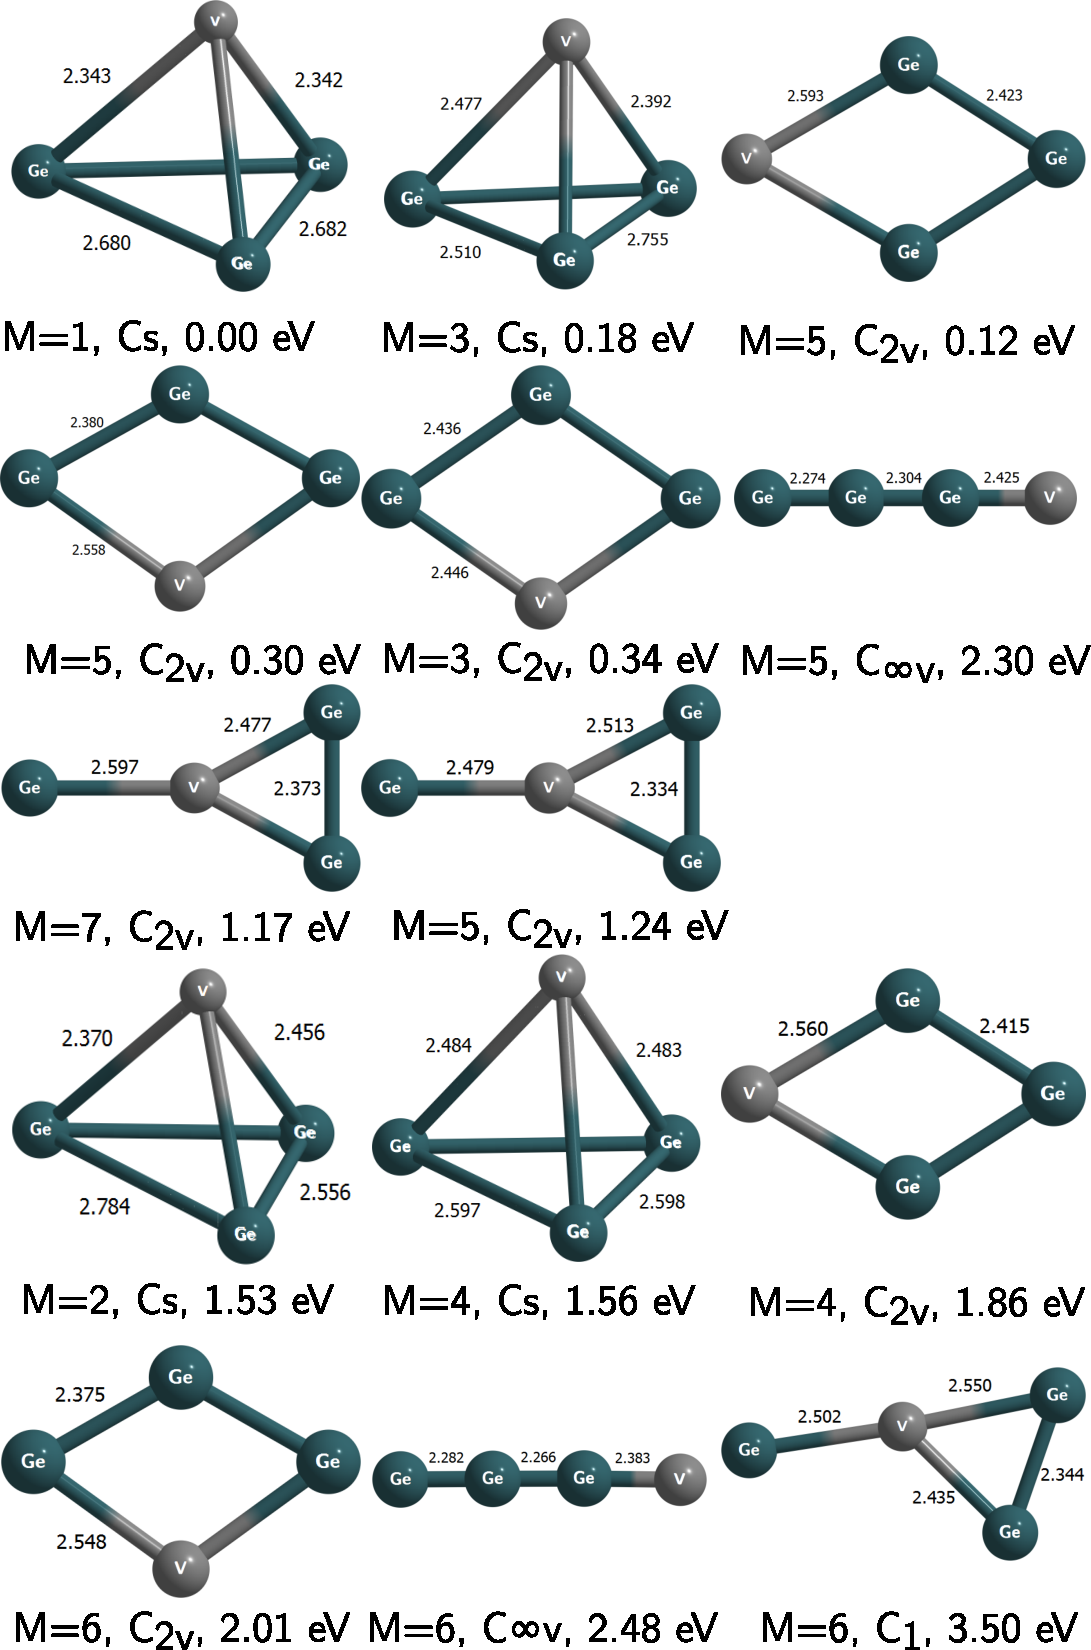
\includegraphics[width=0.8\textwidth]{stable-isomers}
	\caption{Relative energies (eV) of several \ch{VGe3^{-/0}} isomers roughly estimated using the \acrshort{dft}/M06-L functional.}
	\label{a5fig:isomers}
\end{figure}




\begin{table}[htbp!]
	\centering
	\caption{Comparison of three functionals B3LYP, M06L and BP86 in terms of calculated \acrshort{ade} and \acrshort{vde} for the band X. The \acrshort{ade}s are in parentheses}
	\label{a5tbl:selectFun}
	\begin{tabular}{@{}ccccc@{}}
	\toprule
	transition & \multicolumn{4}{c}{\acrshort{vde} and \acrshort{ade} (eV)} \\ \midrule
			                    & B3LYP   & M06L    & BP86    & expt.  \\
	$^1$A$_1$ $\longrightarrow$ 1$^2$A'   & 1.70    & 1.61    & 1.93    & 2.02   \\
			                    & (1.61)  & (1.51)  & (1.88)  & (1.73) \\
	$^1$A$_1$ $\longrightarrow$ 1$^2$A"   & 1.70    & 1.62    & 1.94    &        \\
			                    & (1.61)  & (1.52)  & (1.89)  &        \\ \bottomrule
	\end{tabular}
	\end{table}



Obviously, both B3LYP and M06L give underestimation to \acrshort{ade} and \acrshort{vde} of the band X in comparison the experimental values. On the other hand, BP86 reproduces these values quite well. Therefore, in this work the BP86 functional is used.




\begin{table}[htbp!]
	\centering 
	\caption{Equilibrium geometries and harmonic vibrational frequencies of three states being involved in the band X obtained at the BP86 level. Only vibrations with intensities larger than zero are considered for the simulations}
	\label{a5tbl:freq}
	\begin{tabular}{@{}ccccc@{}}
	\toprule
	state & \begin{tabular}[c]{@{}c@{}}geometry (\AA) \\ r$_1$, r$_2$, r$_3$, r$_4$\end{tabular} & \begin{tabular}[c]{@{}c@{}}vibrational frequency \\ (cm$^{-1}$)\end{tabular} & band & ionization 					\\ \midrule
	$^1$A$_1$   & 2.33, 2.33, 2.70, 2.70      & 123,124, 183, 276, 276, 376  &      &            					\\
	1$^2$A'     & 2.46, 2.56, 2.80, 3.04      & 75, 120, 181, 229, 260, 337  & X    & $^1$A$_1$ $\longrightarrow$ 1$^2$A'   \\
	1$^2$A"     & 2.33, 2.39, 2.73, 2.54      & 138, 186, 211, 266, 338      & X    & $^1$A$_1$ $\longrightarrow$ 1$^2$A"   \\ \bottomrule
	\end{tabular}
	\end{table}





\begin{center}
\begin{landscape}
\begin{longtable}{@{}clllllrrr@{}}
	\caption{Optimized cartesian coordinates and symmetric vibrational frequencies of the anionic and neutral ground states obtained at the \acrshort{caspt2} level of theory} \\
	\toprule
	isomer  & state    & sym.  	&  & symmetric vibrational frequency     & \multicolumn{4}{c}{Cartesian coordinate (\AA)}      \\ \midrule 
	\endfirsthead
	\multicolumn{6}{c}%
	{{\tablename\ \thetable{} -- continued from previous page}} \\
	\toprule
	isomer  & state    & sym.  	&  & symmetric vibrational frequency     & \multicolumn{4}{c}{Cartesian coordinate (\AA)}     \\ \midrule 
	\endhead
	\bottomrule \multicolumn{6}{r}{{Continued on next page}} \\   
	\endfoot	
	\bottomrule 
	\endlastfoot	
tetrahedral $\eta^3$-\ch{(Ge3)V-} & $^1$A'  & C$_s$  &  & 115, 191, 279, 360  & V   &   0.00000000  &  -0.06765893  &  -0.00399809 \\
                    &       &      &  &                                      & Ge  &   0.00000000  &  -1.83345246  &  -1.55563418 \\
                    &       &      &  &                                      & Ge  &   1.35187933  &  -1.81730861  &   0.78865227 \\
                    &       &      &  &                                      & Ge  &  -1.35187933  &  -1.81730861  &   0.78865227 \\
	& $^1$A"        & C$_s$        &  & 137, 185, 256, 323                   & V   &   0.00000000  &  -0.00161078  &  -0.04433521 \\
                    &       &      &  &                                      & Ge  &   0.00000000  &  -1.82304694  &  -1.55795060 \\
                    &       &      &  &                                      & Ge  &   1.25745054  &  -1.89376228  &   0.83130581 \\
                    &       &      &  &                                      & Ge  &  -1.25745054  &  -1.89376228  &   0.83130581 \\
	& $^3$A'        & C$_s$        &  & 116, 168, 220, 331                   & V   &   0.00000000  &   0.00533299  &   0.05427522 \\
                    &       &      &  &                                      & Ge  &   0.00000000  &  -1.90390730  &  -1.49908775 \\
                    &       &      &  &                                      & Ge  &   1.41586144  &  -1.81984568  &   0.67383253 \\
                    &       &      &  &                                      & Ge  &  -1.41586144  &  -1.81984568  &   0.67383253 \\
	& $^3$A"        & C$_s$        &  & 115, 190, 263, 345                   & V   &   0.00000000  &  -0.01152144  &  -0.04596821 \\
                    &       &      &  &                                      & Ge  &   0.00000000  &  -1.81841103  &  -1.58520464 \\
                    &       &      &  &                                      & Ge  &   1.25859948  &  -1.88848754  &   0.86019285 \\
                    &       &      &  &                                      & Ge  &  -1.25859948  &  -1.88848754  &   0.86019285 \\
	& $^5$A'        & C$_s$        &  & 70, 138, 184, 302                    & V   &   0.00000000  &   0.08546897  &   0.03882591 \\
                    &       &      &  &                                      & Ge  &   0.00000000  &  -1.91905492  &  -1.50314117 \\
                    &       &      &  &                                      & Ge  &   1.35473113  &  -1.88483404  &   0.69333526 \\
                    &       &      &  &                                      & Ge  &  -1.35473113  &  -1.88483404  &   0.69333526 \\
	& $^5$A"        & C$_s$        &  & 103, 198, 217, 311                   & V   &   0.00000000  &   0.13317496  &   0.01267973 \\
                    &       &      &  &                                      & Ge  &   0.00000000  &  -1.91480324  &  -1.50218609 \\
                    &       &      &  &                                      & Ge  &   1.27904906  &  -1.93679172  &   0.71852636 \\
                    &       &      &  &                                      & Ge  &  -1.27904906  &  -1.93679172  &   0.71852636 \\
rhombic $\eta^2$-\ch{(Ge3)V-}& $^5$B$_2$  & C$_{2v}$ &  & 178, 211, 312       & V   &   0.00000000  &   0.00000000  &  -0.11460949 \\
		            &       &      &  &                                      & Ge  &   0.00000000  &   0.00000000  &   4.22941386 \\
		            &       &      &  &                                      & Ge  &   0.00000000  &   1.28426245  &   2.18250462 \\
		            &       &      &  &                                      & Ge  &   0.00000000  &  -1.28426245  &   2.18250462 \\
   & $^5$A$_2$      & C$_{2v}$     &  & 136, 203, 295                        & V   &   0.00000000  &   0.00000000  &  -0.15180644 \\
		            &       &      &  &                                      & Ge  &   0.00000000  &   0.00000000  &   4.24746929 \\
		            &       &      &  &                                      & Ge  &   0.00000000  &   1.29332407  &   2.20164615 \\
		            &       &      &  &                                      & Ge  &   0.00000000  &  -1.29332407  &   2.20164615 \\
cyclic $\eta^3$-\ch{(Ge3)V-} & $^1$A$_1$ & C$_{2v}$ &  & 151, 213, 285        & V   &   0.00000000  &   0.00000000  &  -0.13064578 \\
		            &       &      &  &                                      & Ge  &   0.00000000  &   0.00000000  &   2.61238541 \\
		            &       &      &  &                                      & Ge  &   0.00000000  &   1.97629995  &   1.20921648 \\
		            &       &      &  &                                      & Ge  &   0.00000000  &  -1.97629995  &   1.20921648 \\
   & $^3$B$_2$      & C$_{2v}$     &  & 144, 180, 258                        & V   &   0.00000000  &   0.00000000  &  -0.05504545 \\
		            &       &      &  &                                      & Ge  &   0.00000000  &   0.00000000  &   2.57623254 \\
		            &       &      &  &                                      & Ge  &   0.00000000  &   2.03380523  &   1.16976903 \\
		            &       &      &  &                                      & Ge  &   0.00000000  &  -2.03380523  &   1.16976903 \\
   & $^3$A$_2$      & C$_{2v}$     &  & 146, 184, 279                        & V   &   0.00000000  &   0.00000000  &  -0.10171853 \\
		            &       &      &  &                                      & Ge  &   0.00000000  &   0.00000000  &   2.61325554 \\
		            &       &      &  &                                      & Ge  &   0.00000000  &   2.01515598  &   1.17941912 \\
		            &       &      &  &                                      & Ge  &   0.00000000  &  -2.01515598  &   1.17941912 \\
   & $^5$A$_1$      & C$_{2v}$     &  & 68, 197, 258                         & V   &   0.00000000  &   0.00000000  &  -0.21786494 \\
		            &       &      &  &                                      & Ge  &   0.00000000  &   0.00000000  &   2.68566027 \\
		            &       &      &  &                                      & Ge  &   0.00000000  &   1.95588328  &   1.22316079 \\
		            &       &      &  &                                      & Ge  &   0.00000000  &  -1.95588328  &   1.22316079 \\
   & $^5$B$_1$     & C$_{2v}$      &  & 87, 229, 265                         & V   &   0.00000000  &   0.00000000  &  -0.39863468 \\
		            &       &      &  &                                      & Ge  &   0.00000000  &   0.00000000  &   2.85036610 \\
		            &       &      &  &                                      & Ge  &   0.00000000  &   1.82145020  &   1.23922471 \\
		            &       &      &  &                                      & Ge  &   0.00000000  &  -1.82145020  &   1.23922471 \\
   & $^5$B$_2$   & C$_{2v}$        &  & 179, 198, 269                        & V   &   0.00000000  &   0.00000000  &  -0.10123254 \\
		            &       &      &  &                                      & Ge  &   0.00000000  &   0.00000000  &   2.54186846 \\
		            &       &      &  &                                      & Ge  &   0.00000000  &   2.04416154  &   1.25032020 \\
		            &       &      &  &                                      & Ge  &   0.00000000  &  -2.04416154  &   1.25032020 \\
tetrahedral $\eta^3$-\ch{(Ge3)V}& $^2$A' & C$_s$  &  & 123, 179, 233, 342     & V   &   0.00000000  &  -0.02016065  &   0.04254654 \\
			        &       &      &  &                                      & Ge  &   0.00000000  &  -1.88624413  &  -1.49909433 \\
			        &       &      &  &                                      & Ge  &   1.39293469  &  -1.81201522  &   0.68556779 \\
			        &       &      &  &                                      & Ge  &  -1.39293469  &  -1.81201522  &   0.68556779 \\
	& $^2$A"        & C$_s$        &  & 152, 210, 254, 348                   & V   &   0.00000000  &  -0.03597573  &  -0.04192480 \\
			        &       &      &  &                                      & Ge  &   0.00000000  &  -1.81343472  &  -1.56976432 \\
			        &       &      &  &                                      & Ge  &   1.26511375  &  -1.86900955  &   0.84070913 \\
			        &       &      &  &                                      & Ge  &  -1.26511375  &  -1.86900955  &   0.84070913 \\
	& $^4$A' 		& C$_s$        &  & 111, 170, 221, 311                   & V   &   0.00000000  &   0.04168830  &   0.02116877 \\
			        &       &      &  &                                      & Ge  &   0.00000000  &  -1.89017746  &  -1.50321583 \\
			        &       &      &  &                                      & Ge  &   1.35803991  &  -1.86993084  &   0.71106706 \\
			        &       &      &  &                                      & Ge  &  -1.35803991  &  -1.86993084  &   0.71106706 \\
	& $^4$A" 	    & C$_s$        &  & 109, 166, 196, 298                   & V   &   0.00000000  &   0.06206101  &   0.00269158 \\
			        &       &      &  &                                      & Ge  &   0.00000000  &  -1.88206833  &  -1.51520425 \\
			        &       &      &  &                                      & Ge  &   1.30510443  &  -1.89841267  &   0.74153267 \\
			        &       &      &  &                                      & Ge  &  -1.30510443  &  -1.89841267  &   0.74153267 \\
	& $^6$A'     	& C$_s$ 	   &  & 54,  90, 206, 284                    & V   &   0.00000000  &   0.19171890  &   0.20363904 \\
			        &       &      &  &                                      & Ge  &   0.00000000  &  -2.13820200  &  -1.34689356 \\
			        &       &      &  &                                      & Ge  &   1.64225032  &  -1.77193690  &   0.37227452 \\
			        &       &      &  &                                      & Ge  &  -1.64225032  &  -1.77193690  &   0.37227452 \\
	& $^6$A"     	& C$_s$        &  & 85, 156, 173, 289                    & V   &   0.00000000  &   0.15796319  &  -0.02264408 \\
			        &       &      &  &                                      & Ge  &   0.00000000  &  -1.88296649  &  -1.47276529 \\
			        &       &      &  &                                      & Ge  &   1.31838003  &  -1.99341671  &   0.72442936 \\
				    &       &      &  &                                      & Ge  &  -1.31838003  &  -1.99341671  &   0.72442936 \\
rhombic $\eta^2$-\ch{(Ge3)V} & $^4$B$_2$ & C$_{2v}$  &  & 186, 288, 452       & V   &   0.00000000  &   0.00000000  &  -0.01032115 \\
					&       &      &  &                                      & Ge  &   0.00000000  &   0.00000000  &   4.20004542 \\
					&       &      &  &                                      & Ge  &   0.00000000  &   1.26182801  &   2.10758473 \\
					&       &      &  &                                      & Ge  &   0.00000000  &  -1.26182801  &   2.10758473 \\
	& $^4$A$_2$  	& C$_{2v}$     &  & 152, 276, 290                        & V   &   0.00000000  &   0.00000000  &   0.00204626 \\
					&       &      &  &                                      & Ge  &   0.00000000  &   0.00000000  &   4.15404480 \\
					&       &      &  &                                      & Ge  &   0.00000000  &   1.33378418  &   2.14121794 \\
					&       &      &  &                                      & Ge  &   0.00000000  &  -1.33378418  &   2.14121794 \\
cyclic $\eta^3$-\ch{(Ge3)V} & $^2$B$_2$ & C$_{2v}$  &  & 153, 195, 308        & V   &   0.00000000  &   0.00000000  &  -0.00256885 \\
					&       &      &  &                                      & Ge  &   0.00000000  &   0.00000000  &   2.54879242 \\
					&       &      &  &                                      & Ge  &   0.00000000  &   2.06223030  &   1.14473144 \\
					&       &      &  &                                      & Ge  &   0.00000000  &  -2.06223030  &   1.14473144 \\
	& $^4$B$_1$     & C$_{2v}$     &  & 102, 207, 295                        & V   &   0.00000000  &   0.00000000  &  -0.18586040 \\
					&       &      &  &                                      & Ge  &   0.00000000  &   0.00000000  &   2.65841018 \\
					&       &      &  &                                      & Ge  &   0.00000000  &   1.97345697  &   1.21840634 \\
					&       &      &  &                                      & Ge  &   0.00000000  &  -1.97345697  &   1.21840634 \\
	& $^4$B$_2$     & C$_{2v}$     &  & 140, 174, 299                        & V   &   0.00000000  &   0.00000000  &  -0.06883400 \\
					&       &      &  &                                      & Ge  &   0.00000000  &   0.00000000  &   2.49284775 \\
					&       &      &  &                                      & Ge  &   0.00000000  &   2.07258724  &   1.26694237 \\
					&       &      &  &                                      & Ge  &   0.00000000  &  -2.07258724  &   1.26694237 \\
	& $^6$A$_1$     & C$_{2v}$     &  & 105, 181, 269                        & V   &   0.00000000  &   0.00000000  &  -0.13421284 \\
					&       &      &  &                                      & Ge  &   0.00000000  &   0.00000000  &   2.50503653 \\
					&       &      &  &                                      & Ge  &   0.00000000  &   2.06634839  &   1.32013243 \\
					&       &      &  &                                      & Ge  &   0.00000000  &  -2.06634839  &   1.32013243 \\ 
\label{a5tbl:geometries} 
\end{longtable}
\end{landscape}
\end{center}



